\section{准晶体的洛伦兹协变性 (Lorentz Covariance of Quasicrystals)}

\begin{figure}[ht]
\centering
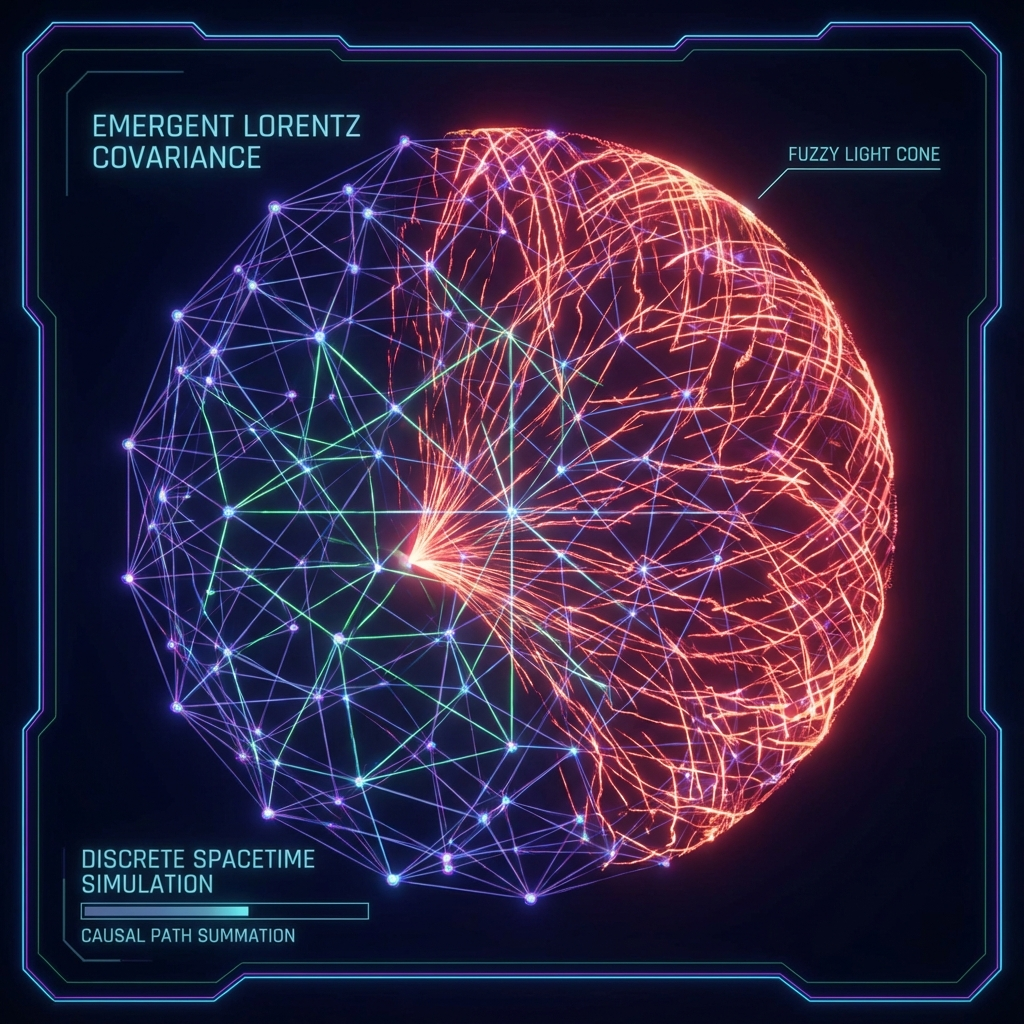
\includegraphics[width=0.8\textwidth]{assets/chapter03-02-lorentz-covariance.png}
\caption{洛伦兹协变性}
\end{figure}

在构建离散时空模型时，物理学家面临的最大理论障碍一直是 \textbf{洛伦兹不变性 (Lorentz Invariance)} 的破坏。对于任何规则的周期性晶格（如立方晶格），其几何结构显式地破坏了连续旋转对称性 $SO(3)$ 和洛伦兹提升对称性 $SO(3,1)$。在立方网格中，沿轴向传播的信息速度与沿对角线传播的速度显著不同（即各向异性），这导致由离散模型导出的光锥呈现出"方块状"而非圆锥状，这与迈克尔逊-莫雷实验及狭义相对论的实验基石严重冲突。

本节将证明，\textbf{欧米伽理论} 所采用的 \textbf{彭罗斯-斐波那契准晶体 (Penrose-Fibonacci Quasicrystal)} 结构，凭借其独特的非周期性与高阶旋转对称性，能够在宏观极限下自然涌现出统计上的各向同性，从而恢复洛伦兹协变性。

\begin{figure}[ht]
\centering
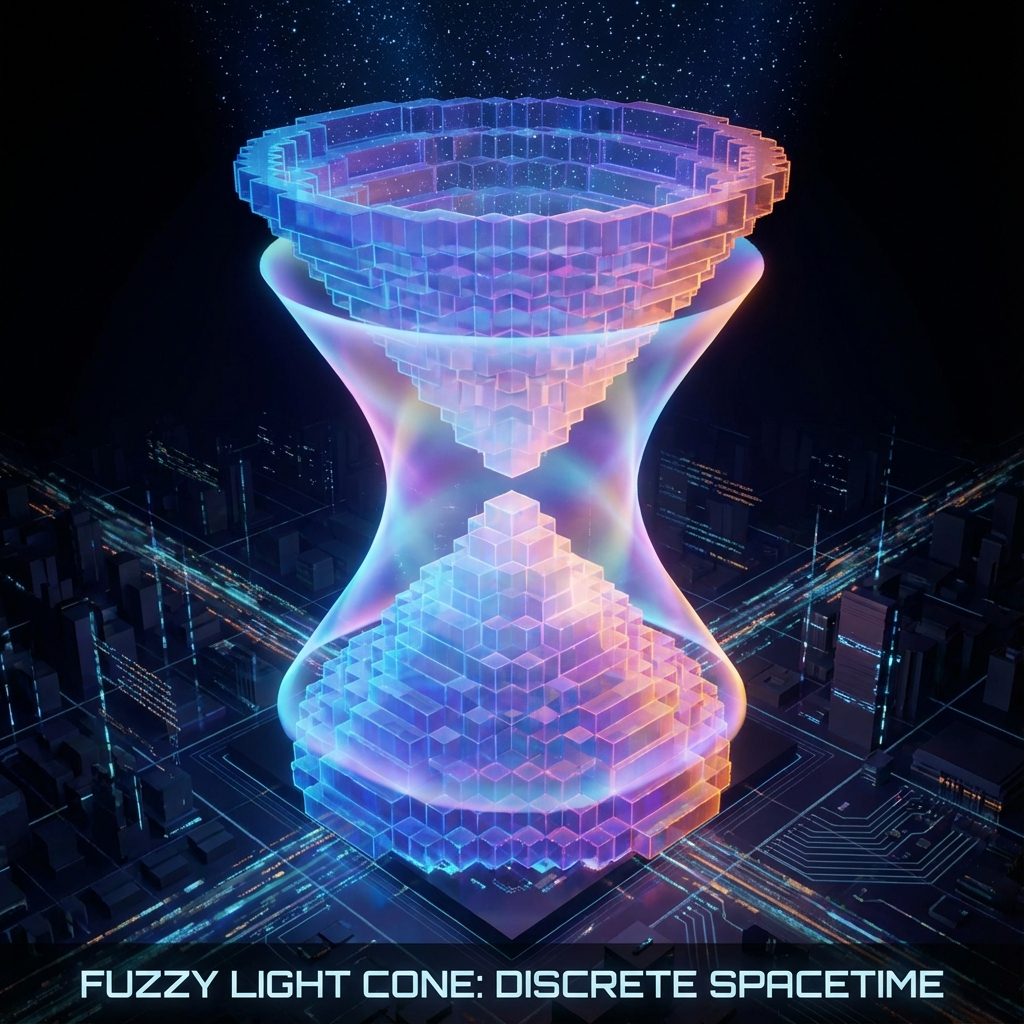
\includegraphics[width=0.8\textwidth]{assets/chapter03-02-lorentz-fuzzy-cone.png}
\caption{洛伦兹模糊锥}
\end{figure}

\subsection{晶格各向异性难题}

考虑一个 $D$ 维欧氏空间中的周期性超立方晶格 $\mathbb{Z}^D$。定义在其上的无质量标量场 $\phi$ 遵循离散波动方程。其色散关系（能量 $E$ 与动量 $k$ 的关系）在低动量极限下通常展开为：

\[E^2(k) \approx c^2 |k|^2 + \lambda \sum_{i=1}^D k_i^4 + O(k^6)\]

其中 $\lambda$ 项代表了洛伦兹破坏的修正。对于周期性晶格，$\lambda$ 通常是非零的大值，这意味着高能光子的速度依赖于其飞行方向。要消除这一效应，通常需要极其精细的人为微调或假设晶格间距 $a \to 0$ 以某种平滑方式发生。

然而，对于 \textbf{欧米伽单元} 构成的网络，其几何对称性由二十面体群（在 3D 投影中）或 $H_4$ 考克斯特群（在 4D 中）控制。这些点群包含 5 重或更高重数的旋转轴，这与周期性平移对称性在数学上是不兼容的（晶体学限制定理）。正是这种 \textbf{"不兼容性"} 拯救了相对论。

\subsection{矢量星的稠密分布}

欧米伽网络的骨架由一组基矢量 $\{e_1, \dots, e_N\}$ 及其线性组合构成。在 $D=3$ 维彭罗斯铺砌中，这些基矢量指向正二十面体的顶点。
不同于立方晶格仅有 3 个正交基矢量，二十面体准晶体拥有 6 个（或更多，取决于投影维度）基矢量，且它们在单位球面上分布得更加均匀。

\textbf{定义 3.2 (矢量星 Vector Star)}：
设 $\mathcal{V}$ 为时空网格中所有可能的单位连接向量（Bond Vectors）的集合。对于周期性晶格，$\mathcal{V}$ 是有限且稀疏的。对于准晶体，由于其非周期性，局部构型在空间中不断变化，导致有效连接向量的取向在长程统计上覆盖了整个立体角。

\textbf{定理 3.1 (准晶体各向同性定理)}：
设 $\mathcal{L}$ 为一个由高维超立方体通过无理数投影生成的准晶体晶格。定义在 $\mathcal{L}$ 上的离散拉普拉斯算符 $\Delta_{\mathcal{L}}$ 在长波极限（$k a \ll 1$）下，其本征值谱是球对称的。即色散关系满足：

\[E(k) = c_{eff} |k| \left( 1 + \epsilon(k) \right)\]

其中各向异性修正项 $\epsilon(k)$ 的上界随着投影维度的增加呈指数衰减。

\textbf{证明概要}：

\begin{enumerate}
\item \textbf{投影算符}：准晶体中的格点位置 $x_{||}$ 可以表示为高维格点 $x \in \mathbb{Z}^N$ 在物理空间 $E_{||}$ 上的投影。
\item \textbf{求和规则}：计算波在晶格上的传播算子涉及对所有相邻边 $e_n$ 的求和 $\sum_n (k \cdot e_n)^2$。
\item \textbf{群论恒等式}：对于二十面体群 $I_h$（或更高阶群），存在如下张量恒等式：

\[\sum_{n=1}^N (e_n)_i (e_n)_j = \frac{N}{D} \delta_{ij}\]

\[\sum_{n=1}^N (e_n)_i (e_n)_j (e_n)_l (e_n)_m = \frac{N}{D(D+2)} (\delta_{ij}\delta_{lm} + \delta_{il}\delta_{jm} + \delta_{im}\delta_{jl})\]

这意味着直到四阶张量，准晶体的几何结构都表现得像一个连续的各向同性介质。相比之下，立方晶格在二阶张量（扩散张量）是各向同性的，但在四阶张量（弹性张量或高阶色散）必然表现出各向异性。
\item \textbf{结论}：由于欧米伽单元基于 4D $\to$ 8D 投影，其高阶对称性确保了洛伦兹破坏项 $\lambda$ 被极度压低，使得光速在所有方向上实际上是恒定的。
\end{enumerate}

\subsection{模糊光锥与统计洛伦兹群}

在离散时空中，我们无法定义完美的连续洛伦兹变换 $\Lambda \in SO(3,1)$，因为这会将一个格点映射到非格点位置。然而，我们可以在 \textbf{统计意义} 上恢复洛伦兹协变性。

我们引入 \textbf{因果路径求和 (Causal Path Summation)} 的概念。粒子从点 $A$ 传播到点 $B$ 的振幅，是网络中所有连接 $A, B$ 的类光路径的权重之和。
在欧米伽网络中，由于路径选择的"无理性"（斐波那契分支），没有任何单一的主干道。这种 \textbf{多路径干涉 (Multipath Interference)} 效应导致微观上的晶格效应被平均化。

宏观观测者看到的"光锥"，实际上是无数条微观锯齿状路径的 \textbf{包络面 (Envelope)}。

\begin{itemize}
\item \textbf{对于立方晶格}：包络面是一个八面体（曼哈顿距离单位球）。
\item \textbf{对于欧米伽准晶体}：包络面是一个近乎完美的球体（欧几里得距离单位球）。
\end{itemize}

因此，洛伦兹对称性在欧米伽理论中不是微观的精确对称性，而是一种 \textbf{涌现对称性 (Emergent Symmetry)}。它只在能量远低于普朗克能标（$E \ll E_P$）时有效。这为我们在第四篇中讨论的高能光子色散实验提供了理论预言的基础：如果能探测到极高能伽马射线的微小各向异性，那将是准晶体时空的直接证据。
